% Physics-informed identification of coupled beam--RF feedback dynamics from closed-loop measurements
% in a storage ring.  REVTeX 4.2, Physical Review Accelerators and Beams style.
% Build: pdflatex main; bibtex main; pdflatex main; pdflatex main   (or latexmk -pdf main.tex)
% Figures in ./figures and numbers.tex, table_*.tex are generated by ../code/make_figures.py and ../code/make_numbers.py.
\documentclass[aps,prab,twocolumn,superscriptaddress,nofootinbib,floatfix]{revtex4-2}

\usepackage[utf8]{inputenc}
\usepackage[T1]{fontenc}
\usepackage{amsmath,amssymb,bm}
\usepackage{graphicx}
\usepackage{booktabs}
\usepackage{dcolumn}
\usepackage[detect-all]{siunitx}
\usepackage{xcolor}
\usepackage{tikz}
\usetikzlibrary{arrows.meta,positioning,calc,fit}
\usepackage[colorlinks=true,linkcolor=blue!50!black,citecolor=blue!50!black,urlcolor=blue!50!black]{hyperref}

\newcommand{\vect}[1]{\bm{#1}}
\newcommand{\mat}[1]{\mathbf{#1}}
\newcommand{\fRF}{f_\mathrm{RF}}
\newcommand{\wRF}{\omega_\mathrm{RF}}
\newcommand{\Ib}{I_b}
\newcommand{\gA}{g_A}
\newcommand{\kAP}{k_\mathrm{AP}}
\newcommand{\QL}{Q_L}
\newcommand{\arad}{\alpha_\mathrm{rad}}
\renewcommand{\Re}{\operatorname{Re}}
\renewcommand{\Im}{\operatorname{Im}}
\raggedbottom

% generated by code/make_numbers.py
\newcommand{\Gzero}{1.39}
\newcommand{\GzeroErr}{0.01}
\newcommand{\QLFit}{6681}
\newcommand{\QLFitErr}{12}
\newcommand{\QLSelNom}{6184}
\newcommand{\alphaSpread}{17}
\newcommand{\alphaSpreadFree}{71}
\newcommand{\alphacAboveHi}{28}
\newcommand{\alphacAboveLo}{20}
\newcommand{\alphacFit}{1.412}
\newcommand{\alphacFitErr}{0.003}
\newcommand{\alphacHi}{1.44}
\newcommand{\alphacKs}{1.40}
\newcommand{\alphacLo}{1.37}
\newcommand{\ampLoopHigh}{0.43}
\newcommand{\chainEvenPh}{3.7}
\newcommand{\chainOdd}{0.77}
\newcommand{\chiBeamEff}{4.71}
\newcommand{\chiBeamEffAc}{4.71}
\newcommand{\chiBeamFree}{0.70}
\newcommand{\chiBeamGlobalFree}{0.78}
\newcommand{\chiBeamNobeam}{4.89}
\newcommand{\chiBeamOne}{0.79}
\newcommand{\chiBeamSel}{0.71}
\newcommand{\chiBeamSelNom}{1.86}
\newcommand{\chiBeamShared}{5.56}
\newcommand{\chiBeamSpread}{5.97}
\newcommand{\chiBeamTrip}{0.92}
\newcommand{\chiCostKap}{351}
\newcommand{\chiCostKapPct}{1.4}
\newcommand{\chiEff}{1.406}
\newcommand{\chiEffAc}{1.406}
\newcommand{\chiFree}{1.002}
\newcommand{\chiGlobalFree}{1.098}
\newcommand{\chiKs}{1.0148}
\newcommand{\chiNobeam}{1.569}
\newcommand{\chiOne}{1.101}
\newcommand{\chiSel}{1.016}
\newcommand{\chiSelNom}{1.250}
\newcommand{\chiShared}{15.462}
\newcommand{\chiSpread}{14.937}
\newcommand{\chiTrip}{1.176}
\newcommand{\chiWideEff}{0.95}
\newcommand{\chiWideEffAc}{0.95}
\newcommand{\chiWideFree}{1.04}
\newcommand{\chiWideGlobalFree}{1.14}
\newcommand{\chiWideNobeam}{1.11}
\newcommand{\chiWideOne}{1.14}
\newcommand{\chiWideSel}{1.06}
\newcommand{\chiWideSelNom}{1.16}
\newcommand{\chiWideShared}{16.79}
\newcommand{\chiWideSpread}{16.13}
\newcommand{\chiWideTrip}{1.21}
\newcommand{\condAll}{9.9\times10^{4}}
\newcommand{\condOne}{3.7\times10^{5}}
\newcommand{\condOneW}{2.1\times10^{6}}
\newcommand{\condScan}{2.0\times10^{5}}
\newcommand{\cvGainEff}{1.91}
\newcommand{\cvGainFree}{1.35}
\newcommand{\cvGainIn}{0.83}
\newcommand{\cvGainOne}{1.42}
\newcommand{\cvGainSel}{1.37}
\newcommand{\cvGainShared}{28.77}
\newcommand{\cvIaEff}{2.65}
\newcommand{\cvIaFree}{0.95}
\newcommand{\cvIaIn}{0.79}
\newcommand{\cvIaOne}{1.32}
\newcommand{\cvIaSel}{0.92}
\newcommand{\cvIaShared}{12.60}
\newcommand{\cvIbEff}{6.34}
\newcommand{\cvIbFree}{0.82}
\newcommand{\cvIbIn}{0.74}
\newcommand{\cvIbOne}{0.94}
\newcommand{\cvIbSel}{0.78}
\newcommand{\cvIbShared}{3.03}
\newcommand{\cvIcEff}{10.31}
\newcommand{\cvIcFree}{0.63}
\newcommand{\cvIcIn}{0.63}
\newcommand{\cvIcOne}{0.71}
\newcommand{\cvIcSel}{0.69}
\newcommand{\cvIcShared}{12.11}
\newcommand{\cvPhaseEff}{2.22}
\newcommand{\cvPhaseFree}{2.04}
\newcommand{\cvPhaseIn}{2.06}
\newcommand{\cvPhaseOne}{2.44}
\newcommand{\cvPhaseSel}{2.09}
\newcommand{\cvPhaseShared}{25.54}
\newcommand{\daicEff}{9838}
\newcommand{\daicEffAc}{9839}
\newcommand{\daicFree}{\ensuremath{-}339}
\newcommand{\daicGlobalFree}{2047}
\newcommand{\daicNobeam}{13912}
\newcommand{\daicOne}{2132}
\newcommand{\daicSel}{0}
\newcommand{\daicSelNom}{5891}
\newcommand{\daicShared}{363542}
\newcommand{\daicSpread}{350222}
\newcommand{\daicTrip}{4004}
\newcommand{\dampErrHighGain}{165}
\newcommand{\dampHighGainFree}{1.4e3}
\newcommand{\dampHighGainModel}{1.8e3}
\newcommand{\dampHighGainOver}{404}
\newcommand{\dampLowGainFree}{2.4e3}
\newcommand{\dampLowGainModel}{2.3e3}
\newcommand{\dampOverRatio}{2.4}
\newcommand{\dbicEff}{10147}
\newcommand{\dbicEffAc}{10156}
\newcommand{\dbicFree}{\ensuremath{-}291}
\newcommand{\dbicGlobalFree}{2015}
\newcommand{\dbicNobeam}{13912}
\newcommand{\dbicOne}{2091}
\newcommand{\dbicSel}{0}
\newcommand{\dbicSelNom}{5883}
\newcommand{\dbicShared}{363445}
\newcommand{\dbicSpread}{350189}
\newcommand{\dbicTrip}{3955}
\newcommand{\dchiEff}{9762}
\newcommand{\dchiEffAc}{9761}
\newcommand{\dchiFree}{\ensuremath{-}351}
\newcommand{\dchiGlobalFree}{2055}
\newcommand{\dchiNobeam}{13912}
\newcommand{\dchiOne}{2142}
\newcommand{\dchiOneHigh}{184}
\newcommand{\dchiOneLow}{1124}
\newcommand{\dchiOneMid}{834}
\newcommand{\dchiSel}{0}
\newcommand{\dchiSelNom}{5893}
\newcommand{\dchiShared}{363566}
\newcommand{\dchiSpread}{350230}
\newcommand{\dchiTrip}{4016}
\newcommand{\driveHigh}{29}
\newcommand{\driveLow}{28}
\newcommand{\driveMargin}{4.4}
\newcommand{\driveSat}{80}
\newcommand{\driveSet}{28}
\newcommand{\fsFit}{10.97}
\newcommand{\fsFitErr}{0.01}
\newcommand{\fsHi}{11.1}
\newcommand{\fsLo}{10.8}
\newcommand{\fsNom}{10.03}
\newcommand{\fsRatio}{9}
\newcommand{\gaAllAt}{1967}
\newcommand{\gaAllHi}{0.36}
\newcommand{\gaAllLo}{0.35}
\newcommand{\gaAllOpt}{0.35}
\newcommand{\gaFreeHi}{0.78}
\newcommand{\gaFreeHigh}{0.35}
\newcommand{\gaFreeLo}{0.35}
\newcommand{\gaOneAt}{98}
\newcommand{\gaOneHi}{0.38}
\newcommand{\gaOneKly}{0.32}
\newcommand{\gaOneKlyErr}{0.01}
\newcommand{\gaOneLo}{0.30}
\newcommand{\gaOneOpt}{0.30}
\newcommand{\gaOneWAt}{7}
\newcommand{\gaOneWHi}{0.76}
\newcommand{\gaOneWLo}{0.29}
\newcommand{\gaOneWOpt}{0.32}
\newcommand{\gaScanAt}{466}
\newcommand{\gaScanHi}{0.35}
\newcommand{\gaScanLo}{0.33}
\newcommand{\gaScanOpt}{0.34}
\newcommand{\gaSelHighHi}{0.32}
\newcommand{\gaSelHighLo}{0.31}
\newcommand{\gaSelLow}{0.56}
\newcommand{\gaSelMid}{0.50, 0.39, 0.39}
\newcommand{\gaShiftHigh}{0.05}
\newcommand{\gaTrip}{0.40}
\newcommand{\gaintrackHigh}{107.3}
\newcommand{\gaintrackLow}{107.0}
\newcommand{\halfMedian}{0.75 (range 0.65--0.88)}
\newcommand{\hvpsAHigh}{22.3}
\newcommand{\hvpsALow}{18.8}
\newcommand{\hvpsHigh}{75}
\newcommand{\hvpsLow}{67}
\newcommand{\jointDf}{\ensuremath{-}14}
\newcommand{\jointDfRms}{80}
\newcommand{\jointDs}{+163}
\newcommand{\jointDsRms}{336}
\newcommand{\jointOneDf}{\ensuremath{-}3}
\newcommand{\jointOneDfRms}{100}
\newcommand{\jointOneDs}{+482}
\newcommand{\jointOneDsRms}{598}
\newcommand{\kapAllAt}{125}
\newcommand{\kapAllHi}{\ensuremath{-}0.42}
\newcommand{\kapAllLo}{\ensuremath{-}0.47}
\newcommand{\kapAllOpt}{\ensuremath{-}0.44}
\newcommand{\kapFreeHi}{+0.62}
\newcommand{\kapFreeLo}{\ensuremath{-}0.44}
\newcommand{\kapOneAt}{0}
\newcommand{\kapOneHi}{+0.29}
\newcommand{\kapOneLo}{\ensuremath{-}0.48}
\newcommand{\kapOneOpt}{\ensuremath{-}0.08}
\newcommand{\kapOneWAt}{0}
\newcommand{\kapOneWHi}{+0.62}
\newcommand{\kapOneWLo}{\ensuremath{-}1.00}
\newcommand{\kapOneWOpt}{\ensuremath{-}0.26}
\newcommand{\kapScanAt}{2}
\newcommand{\kapScanHi}{+0.02}
\newcommand{\kapScanLo}{\ensuremath{-}0.17}
\newcommand{\kapScanOpt}{\ensuremath{-}0.08}
\newcommand{\kapTrip}{\ensuremath{-}0.10}
\newcommand{\klyEffHigh}{47}
\newcommand{\klyEffLow}{32}
\newcommand{\klyFwdHigh}{790}
\newcommand{\klyFwdLow}{398}
\newcommand{\klyFwdRatio}{50}
\newcommand{\klyGainDiff}{2.9}
\newcommand{\klyGainHigh}{44.4}
\newcommand{\klyGainLow}{41.5}
\newcommand{\kscale}{0.97}
\newcommand{\kscaleErr}{0.01}
\newcommand{\lowcurChi}{0.59--0.82}
\newcommand{\modeFreeDf}{29}
\newcommand{\modeFreeDs}{173}
\newcommand{\modeFreeFHi}{10.28}
\newcommand{\modeFreeFLo}{8.02}
\newcommand{\modeFreeSHi}{2404}
\newcommand{\modeFreeSLo}{1061}
\newcommand{\nModeRecs}{12}
\newcommand{\nSnapHigh}{6}
\newcommand{\nSnapLow}{3}
\newcommand{\ndata}{25200}
\newcommand{\noiseCorr}{0.9998}
\newcommand{\nparEff}{83}
\newcommand{\nparEffAc}{84}
\newcommand{\nparFree}{51}
\newcommand{\nparGlobalFree}{41}
\newcommand{\nparNobeam}{45}
\newcommand{\nparOne}{40}
\newcommand{\nparSel}{45}
\newcommand{\nparSelNom}{44}
\newcommand{\nparShared}{33}
\newcommand{\nparSpread}{41}
\newcommand{\nparTrip}{39}
\newcommand{\oobEffBand}{6.7}
\newcommand{\oobEffDf}{+198}
\newcommand{\oobEffDfRms}{306}
\newcommand{\oobEffDs}{\ensuremath{-}836}
\newcommand{\oobEffDsRms}{897}
\newcommand{\oobSharedBand}{7.4}
\newcommand{\oobSharedDf}{+378}
\newcommand{\oobSharedDfRms}{533}
\newcommand{\oobSharedDs}{\ensuremath{-}1147}
\newcommand{\oobSharedDsRms}{1184}
\newcommand{\oobWlBand}{7.9}
\newcommand{\oobWlDf}{\ensuremath{-}841}
\newcommand{\oobWlDfRms}{849}
\newcommand{\oobWlDs}{\ensuremath{-}289}
\newcommand{\oobWlDsRms}{439}
\newcommand{\pfwdScale}{0.96}
\newcommand{\tauFit}{635}
\newcommand{\tauFitErr}{1}
\newcommand{\tauSelNom}{645}
\newcommand{\thetaSlopeLow}{1.24}
\newcommand{\thetaSlopeNov}{2.14}
\newcommand{\tripAsymHi}{6.3}
\newcommand{\tripAsymLo}{1.2}
\newcommand{\tripCohHi}{0.98}
\newcommand{\tripCohLo}{0.93}
\newcommand{\tripDelay}{189}
\newcommand{\tripDriveDiff}{3}
\newcommand{\tripFull}{4}
\newcommand{\tripGA}{0.40}
\newcommand{\tripGAErr}{0.05}
\newcommand{\tripGAFull}{0.42}
\newcommand{\tripGAFullErr}{0.02}
\newcommand{\tripGAHigh}{0.34}
\newcommand{\tripGAHighErr}{0.04}
\newcommand{\tripGAHtwo}{0.41}
\newcommand{\tripGALow}{0.44}
\newcommand{\tripGALowErr}{0.02}
\newcommand{\tripGARatio}{0.50}
\newcommand{\tripGARatioErr}{0.06}
\newcommand{\tripGARed}{0.39}
\newcommand{\tripGARedErr}{0.06}
\newcommand{\tripGAmax}{0.44}
\newcommand{\tripGAmin}{0.30}
\newcommand{\tripKAP}{\ensuremath{-}0.10}
\newcommand{\tripKAPErr}{0.05}
\newcommand{\tripN}{15}
\newcommand{\tripPower}{49}
\newcommand{\tripRatioCohHi}{0.78}
\newcommand{\tripRatioCohLo}{0.66}
\newcommand{\tripReduced}{6}
\newcommand{\tripUsed}{10}
\newcommand{\vkHigh}{75}
\newcommand{\vkLow}{67}
\newcommand{\vkMid}{71, 73, 74}


\begin{document}

\title{Physics-informed identification of coupled beam--RF feedback dynamics\\from closed-loop measurements in a storage ring}

\author{Faya Wang}
\affiliation{SLAC National Accelerator Laboratory, Menlo Park, California 94025, USA}

\date{\today}

\begin{abstract}
The fundamental-mode RF system of an electron storage ring and the stored beam form one coupled dynamical system whose behavior changes with beam current and with the settings of the RF feedback. We ask whether closed-loop measurements made during operation can identify a compact model that predicts these changes. From eighteen closed-loop transfer-function records of the SPEAR3 RF station, taken with its existing noise-injection routine at beam currents from 20 to \SI{500}{mA} and at several loop gains and phases, we identify a physics-informed two-quadrature model of beam, cavities, klystron and feedback. Single records, measured with a one-dimensional excitation, do not determine the klystron's response asymmetry. Records at several loop settings, together with the band of the coupled beam mode, which the routine itself discards, determine its compression but leave its AM/PM conversion correlated with the loop phase; records frozen at trips of the same klystron supply it ($k_\mathrm{AP}=\tripKAP\pm\tripKAPErr$). Of the competing explanations for the large change of the response with beam current---effective linear parameters, unequal cavity detunings, beam dynamics at fixed hardware, and a compressed klystron---only the last describes all records with one set of station constants---at the noise level in the band of the coupled beam mode and to within a few percent across the loop band, with \nparSel{} parameters for \nPoints{} data points---and these constants agree with independent station data. The klystron's compression, its amplitude gain relative to its phase gain, falls from \gaSelLow{} at \SI{22}{mA} to \gaSelHighLo{} at \SI{500}{mA} as the tube, held at a fixed drive, works closer to saturation; at full output the trip records give \tripGAHigh--\tripGAFull. The model predicts records at beam currents it was not trained on almost at in-sample quality, where interpolated effective parameters fail. Its out-of-band prediction of the coupled mode isolates the synchrotron focusing as the one beam parameter the loop band cannot determine; identified from the band of the coupled mode, it implies an incoherent synchrotron frequency \fsRatio\% above the design value, a prediction that a low-current measurement can test.

\end{abstract}

\maketitle

% ======================================================================================================
\section{Introduction}\label{sec:intro}
% ======================================================================================================

In an electron storage ring the fundamental-mode RF system and the stored beam form one coupled dynamical system. The beam induces voltage in the accelerating cavities; the cavities are detuned to compensate the reactive part of that loading; feedback around the klystron lowers the impedance that the beam sees; and the coherent dipole motion of the bunches responds to every perturbation of the gap voltage that the feedback leaves. The classical analyses---Robinson's stability criteria~\cite{Robinson1964}, Pedersen's beam-loaded cavity~\cite{Pedersen1975}, and the treatments of RF feedback by Boussard~\cite{Boussard1985} and Wilson~\cite{Wilson1993}---describe this coupling with a handful of parameters: cavity bandwidth and detuning, loop gain, phase and delay, beam current and synchrotron frequency. Detailed models built on the same physics were used to design and commission the low-level RF (LLRF) systems of PEP-II and the LHC~\cite{Rivetta2007,Mastorides2010}.

At an operating machine, however, several of these parameters are not known well. Components age and are replaced, calibrations are uncertain, parts of the loop setting are not recorded, and the klystron runs close to saturation, where its small-signal response to a change of drive amplitude differs from its response to a change of drive phase. A model assembled from design values may describe one operating point and fail at another. The operational questions---how the damping and frequency of the coherent mode, and the transfer of RF noise to the beam, change with beam current, loop gain and loop phase---call for a model identified from measurements. Such measurements must be made on a running machine: with the feedback closed, with stored beam, with small excitation, and preferably with the diagnostics that already exist~\cite{Forssell1999,Ljung1999}.

This paper asks whether operational closed-loop measurements can identify a compact model that predicts beam--cavity--amplifier--feedback interactions across operating conditions. The approach is physics-informed (grey-box) identification~\cite{Bohlin2006,Pintelon2012}. Physics supplies the structure---cavity resonators, rigid-bunch dipole dynamics, the loop topology and the controller networks, the steady-state beam loading, the way the loop settings enter---and the data determine, and test, the parameters that the physics leaves uncertain. The emphasis is not on fitting one transfer function, which many models do, but on whether one set of physical parameters accounts for the changes of the dynamics as the beam current, the loop gain and the loop phase change, and whether the identified model predicts quantities that were not used to identify it.

The data are the closed-loop responses recorded by the existing routine of the SPEAR3 RF station---band-limited noise injected into the klystron drive and the feedback signal recorded---at beam currents from 20 to \SI{500}{mA} and at several loop gains and phases, in two sessions a month apart, together with records that the station froze at trips of its present klystron. Four features make the problem a stringent test: (i) the excitation is one-dimensional, the same noise sequence on both quadratures, so each record measures a single projection of a response that is not rotation-invariant once the klystron is compressed; (ii) part of the loop phase is not recorded, because a tracking correction drifts by several degrees; (iii) the beam's coherent mode occupies a few kilohertz around $\pm f_s$, a band the routine itself discards; and (iv) independent information on the klystron exists only in those trip records, which are five years older than the closed-loop data.

The paper makes four contributions. Section~\ref{sec:model} gives a two-quadrature (widely linear~\cite{Picinbono1995}) model of the closed loop with beam, including the klystron's compression and AM/PM conversion, and derives what a one-dimensional excitation records. Section~\ref{sec:ident} shows that single records do not determine the klystron's asymmetry, that records taken at different loop settings determine its compression but not its AM/PM conversion, and that the trip records supply the latter. Section~\ref{sec:explain} tests competing explanations for the change of the response with beam current. Section~\ref{sec:valid} validates the selected model by out-of-band prediction of the coupled beam mode, by prediction across operating conditions, and against the klystron compression measured in the trip records; the out-of-band test exposes, and the near band then identifies, the one beam parameter that the loop band cannot determine---the synchrotron frequency.

% ======================================================================================================
\section{The measured system}\label{sec:system}
% ======================================================================================================

\subsection{RF station and direct feedback}

SPEAR3 is a \SI{3}{GeV} storage ring with harmonic number $h=372$ and $\fRF=\SI{476.3}{MHz}$, operated at \SI{500}{mA} in top-off~\cite{Hettel2002,McIntosh2004}. One \SI{1.5}{MW} klystron drives four single-cell PEP-II cavities~\cite{Rimmer1995,Rimmer2000} through a circulator and a waveguide splitter; together they provide $V_\mathrm{RF}=\SI{2.85}{MV}$. Table~\ref{tab:params} lists the parameters used. The cavities are overcoupled and are detuned below $\fRF$ in proportion to the beam current, by about \SI{36}{kHz} at \SI{500}{mA}, to cancel the reactive beam loading; the tuner loops hold the load angle, so the detuning follows the current.

Two cavity and ring constants follow from station snapshots, given the cavities' measured $R/Q=\SI{\RoverQ}{\ohm}$ and $Q_0=\Qzero$~\cite{Rimmer2000}, i.e.\ a shunt impedance $R=V^2/2P=\SI{\Rshunt}{M\ohm}$. Without beam and on tune, the reflection coefficient of each cavity is $(\beta-1)/(\beta+1)$; the snapshots give couplings $\beta=\betaLo$--\betaHi, loaded quality factors $Q_0/(1+\beta)=\QLreflLo$--\QLreflHi, and \QLrefl{} for the vector sum of the four (half-bandwidth \SI{\halfBW}{kHz}); their forward minus reflected power is \wallLo--\wallHi{} times the wall loss $V^2/2R$ computed from the probe voltages. At \SI{500}{mA} the power balance of the four cavities, $\sum_k(P_{\mathrm{fwd},k}-P_{\mathrm{refl},k}-V_k^2/2R)/\Ib$, gives the energy loss per turn $U_0=\UzeroLo$--\SI{\UzeroHi}{MeV}: the \SI{\UzeroDip}{MeV} of the dipoles~\cite{Hettel2002} plus the insertion devices. We use $U_0=\SI{\Uzero}{MeV}$, hence $\phi_s=\ang{\phiS}$ from the crest, and the radiation damping rate $\arad=J_sU_0/(2E_0T_\mathrm{rev})=\SI{\alphaRad}{s^{-1}}$ with $J_s=\Js$, the dipoles' partition number 1.79~\cite{Hettel2002} weighted with 2 for the insertion devices, which sit in dispersion-free straights~\cite{Sands1970}.

The legacy LLRF processor (RFP), an analog VXI module of PEP-II design~\cite{Corredoura1999}, regulates the vector sum of the four probe signals with a direct loop: the measured vector sum is rotated and scaled by a baseband modulator (the loop-phase and loop-gain settings; a frequency-offset tracking correction adds to the phase), the reference is subtracted, and a lead network and a lag (integral) network shape the error before the I/Q modulator that drives the klystron (Fig.~\ref{fig:loop}).

\begin{figure}[tb]
\centering
\resizebox{\columnwidth}{!}{% Block diagram of the measured closed loop with beam (column width).
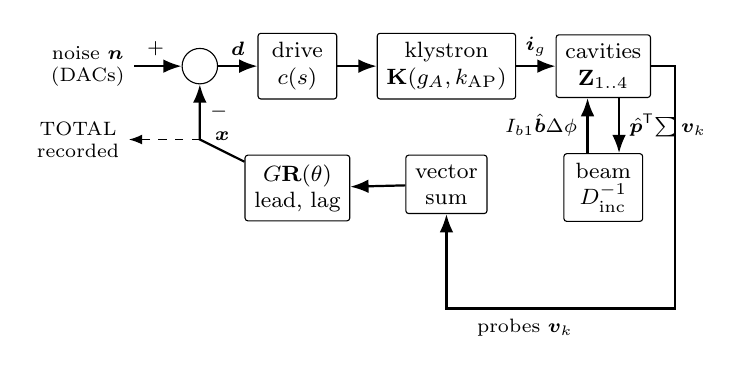
\begin{tikzpicture}[font=\footnotesize, >=Latex, node distance=4mm and 5mm,
  blk/.style={draw, rounded corners=1pt, minimum height=7mm, minimum width=10mm, align=center, fill=white},
  sum/.style={draw, circle, inner sep=0pt, minimum size=4.5mm},
  sig/.style={->, thick},
  lbl/.style={font=\scriptsize, align=center}]
  % forward path
  \node[sum] (s1) {};
  \node[left=6mm of s1, lbl] (n) {noise $\vect n$\\(DACs)};
  \node[blk, right=of s1] (chain) {drive\\$c(s)$};
  \node[blk, right=of chain] (kly) {klystron\\$\mat K(\gA,\kAP)$};
  \node[blk, right=of kly] (cav) {cavities\\$\mat Z_{1..4}$};
  % beam
  \node[blk, below=7mm of cav] (beam) {beam\\$D_\mathrm{inc}^{-1}$};
  % feedback path
  \node[blk, below=7mm of kly] (vs) {vector\\sum};
  \node[blk, below=7mm of chain] (ctrl) {$G\mat R(\theta)$\\lead, lag};
  \node[coordinate, below=7mm of s1] (rec) {};
  \draw[sig] (n) -- node[above, lbl, pos=0.45]{$+$} (s1);
  \draw[sig] (s1) -- node[above, lbl]{$\vect d$} (chain);
  \draw[sig] (chain) -- (kly);
  \draw[sig] (kly) -- node[above, lbl]{$\vect i_g$} (cav);
  \draw[sig] ([xshift=2mm]cav.south) -- node[right, lbl]{$\hat{\vect p}^\mathsf{T}\!\sum\vect v_k$} ([xshift=2mm]beam.north);
  \draw[sig] ([xshift=-2mm]beam.north) -- node[left, lbl]{$I_{b1}\hat{\vect b}\Delta\phi$} ([xshift=-2mm]cav.south);
  \draw[sig] (cav.east) -- ++(3mm,0) |- ([yshift=-11mm]beam.south) -| (vs.south) node[pos=0.25, below, lbl]{probes $\vect v_k$};
  \draw[sig] (vs) -- (ctrl);
  \draw[sig] (ctrl) -- node[above, lbl]{$\vect x$} (rec) -- node[right, lbl]{$-$} (s1);
  \draw[->, dashed] (rec) -- ++(-9mm,0) node[left, lbl]{TOTAL\\recorded};
\end{tikzpicture}
}
\caption{The measured system. Band-limited noise $\vect n$ is added to the klystron drive after the controller; the controller output $\vect x$ is recorded. The beam couples to the four cavities through its dipole motion $\Delta\phi$ [Eq.~\eqref{eq:beam}]; the klystron responds differently to drive amplitude and phase [Eq.~\eqref{eq:klystron}]. Bold symbols are two-quadrature vectors and matrices in the cavity frame.}\label{fig:loop}
\end{figure} The loop delay, measured as \SI{\tauMeas}{ns}~\cite{Sebek2026}, lies mostly in the klystron and the cables to the tunnel. A digital ripple loop acting on the 60-Hz harmonics up to \SI{2.9}{kHz}, and slow EPICS loops for the klystron voltage, the cavity tuners and the gain tracking, complete the system. The klystron-voltage loop holds the drive power at a set point, \SI{\driveSet}{W}, \SI{\driveMargin}{dB} below the saturation setting of \SI{\driveSat}{W}, by moving the HVPS voltage, so the klystron's voltage, and with it its gain, change with the beam current. In the station snapshots the drive is \SI{\driveLow}{W} without beam and \SI{\driveHigh}{W} at \SI{500}{mA}, with the HVPS at \SI{\hvpsLow}{kV} and \SI{\hvpsHigh}{kV}, a klystron gain of \SI{\klyGainLow}{dB} and \SI{\klyGainHigh}{dB}, and an output of \SI{\klyFwdLow}{kW} and \SI{\klyFwdHigh}{kW} at an efficiency of \SI{\klyEffLow}{\percent} and \SI{\klyEffHigh}{\percent}: at the same drive the tube works much closer to saturation with beam than without. Gain tracking holds the product of a DSP coefficient and the measured klystron gain constant; in the same snapshots it is \gaintrackHigh{} at \SI{500}{mA} and \gaintrackLow{} without beam, although the klystron gain differs by \SI{\klyGainDiff}{dB}. The forward-path gain is therefore independent of the operating point, and the loop gain changes only with its setting. Neither the closed-loop records nor the trip records carry the HVPS voltage or the klystron's drive and output power.

\begin{table}[tb]
\caption{Parameters of the SPEAR3 RF station used in the model. Fixed values come from the design report and published measurements~\cite{Hettel2002,Huang2007,Rimmer2000,Corredoura1999} and from station snapshots (Sec.~\ref{sec:system}); identified values are those of Sec.~\ref{sec:explain}.}\label{tab:params}
\footnotesize
\begin{ruledtabular}
\begin{tabular}{lll}
Quantity & Symbol & Value \\
\hline
Energy; harmonic number & $E_0$; $h$ & \SI{3.0}{GeV}; 372 \\
RF frequency & $\fRF$ & \SI{476.304}{MHz} \\
Energy loss per turn (power balance) & $U_0$ & \SI{\Uzero}{MeV} \\
Total gap voltage & $V_\mathrm{RF}$ & \SI{2.85}{MV} \\
Synchronous phase (from crest) & $\phi_s$ & \ang{\phiS} \\
Radiation damping rate & $\arad$ & \SI{\alphaRad}{s^{-1}} \\
Momentum compaction (lattice) & $\alpha_c$ & $1.18\times10^{-3}$ \\
Cavities; $R/Q$; $Q_0$ & $n_\mathrm{cav}$ & 4; \SI{\RoverQ}{\ohm}; \Qzero \\
Lead network zero; pole & & \SI{944}{kHz}; \SI{2.39}{MHz} \\
Lag network zero; pole & & \SI{3.19}{kHz}; \SI{0.26}{kHz} \\
Drive-chain pole & $\omega_a/2\pi$ & \SI{2.5}{MHz} \\
Klystron drive (set; saturation) & $P_\mathrm{d}$ & \SI{\driveSet}{W}; \SI{\driveSat}{W} \\
Klystron AM/PM (trip records) & $\kAP$ & \kapTrip \\
\end{tabular}
\end{ruledtabular}
\end{table}

\subsection{The closed-loop measurement}

The station's closed-loop measurement routine plays a stored sequence of band-limited noise through two DACs whose output is summed into the klystron drive after the controller, and records the controller output: $2^{18}$ complex samples at eight samples per turn (\SI{10.24}{MS/s}, \SI{25.6}{ms}). The stored reference is flat to $\pm\SI{500}{kHz}$. For a complex-linear loop the transfer function from the reference to the record is the complementary sensitivity $-L/(1+L)$. The routine's own estimate discards $\pm\SI{18.8}{kHz}$ around the carrier, the band of the coupled beam mode; here the transfer function is estimated anew from the stored records over the full band (Sec.~\ref{sec:estimation}). The same sequence is stored for the I and Q DACs (correlation \noiseCorr), so the excitation is one-dimensional. The measurement is non-invasive: the injected noise is a fraction of a percent of the drive and the routine runs with stored beam.

\subsection{Data}

Eighteen closed-loop records, taken in two sessions a month apart, are used; Table~\ref{tab:groups} lists them by operating point. Loop-gain and loop-phase settings are given relative to the station's operating settings. In session I the beam current was varied from 20 to \SI{497}{mA} at a loop gain of $\gainSessionOne$~dB, and at \SI{22}{mA} the phase setting was stepped over \ang{\phaseScanLow}. In session II, at about \SI{500}{mA}, the phase setting was lowered by \phaseShiftsHigh{} degrees and the gain by up to \SI{\gainDropMax}{dB}, after one record at \SI{242}{mA}. The frequency-offset tracking correction was on and is not recorded; station snapshots show it varying between \ang{+2} and \ang{+13}.

The trip records are a second, independent data set, of the same klystron, which has been in service since September 2020. At each trip the station freezes, together, the last \SI{5.0}{ms} of the klystron drive and of one cavity probe (both I/Q) and of the klystron output amplitude, all at \SI{10.24}{MS/s}. Of the \tripN{} records of trips in 2021, \tripUsed{} hold RF in every signal: \tripFull{} at full klystron output and \tripReduced{} at \tripPower\% of that power---the output the station needs without beam (\klyFwdRatio\% in the snapshots)---with the same drive to within \tripDriveDiff\%. They carry neither the beam current, nor the loop settings, nor the HVPS voltage.

\subsection{Frequency-response estimation}\label{sec:estimation}

Each record is transformed as a whole. Its discrete Fourier transform, with a resolution of \SI{\lpmBin}{Hz}, obeys at every bin $k$
\begin{equation}\label{eq:lpm}
Y_k=G_kX_k+T_k+V_k,
\end{equation}
where $X$ is the transform of the known excitation, $G$ the frequency response, $T$ a transient that varies smoothly with $k$ (the record is not periodic, so its initial and final conditions leak into every bin) and $V$ the output noise. The local polynomial method (LPM)~\cite{Pintelon2010,Pintelon2012} fits Eq.~\eqref{eq:lpm} by least squares to \lpmBins{} adjacent bins (\SI{\lpmWidth}{Hz}), with $G$ constant and $T$ quadratic in the bin offset. This removes the transient, and neighbourhoods that do not overlap give statistically independent estimates every \SI{\lpmWidth}{Hz}. The expectation of an estimate is a weighted mean of $G$ over its neighbourhood, with weights fixed by the excitation (App.~\ref{app:estimator}); the model is compared with the same weighted mean of its own response, so the comparison is exact even where the coupled mode changes the response within one neighbourhood. The noise variance follows from the residual of a second fit in which $G$ is quadratic as well, averaged over \SI{\lpmSmooth}{kHz}. The estimates are taken in the convention of the routine, the complex conjugate of $Y/X$, which makes the loop delay positive and places the high-current detuning below $\fRF$.

Two bands are distinguished: the \emph{near band}, $|f|<\SI{\fSplit}{kHz}$, which contains the carrier and the coupled mode and which the routine discards, and the \emph{loop band}, $\SI{\fSplit}{kHz}\le|f|\le\SI{\fHi}{kHz}$, where the loop dominates. The neighbourhoods tile the spectrum outward from the carrier; the one centred on it leaves out the carrier bin, which holds the record's mean, the operating point, so the estimates cover the full band without a gap. In the near band every estimate is a data point. In the loop band, where the response is smooth, four (below \SI{100}{kHz}) or eight adjacent estimates are combined with inverse-variance weights into one data point, and the model is evaluated at their mean frequency. Each record thus gives \nCellsRecord{} complex data points over the full band, \nPoints{} real ones for the eighteen records. The real and imaginary parts of the residuals, each divided by its standard deviation, define a Gaussian likelihood, so that $\chi^2/\nu\approx1$ indicates a fit at the noise level and differences of $\chi^2$ are log-likelihood ratios. The scatter of adjacent estimates confirms the predicted variance in the loop band (ratio \calibMedian, App.~\ref{app:estimator}); in the near band, interference lines raise the averaged noise level of the estimates around them, and the ratio lies between \calibNearLo{} and \calibNearHi.

The near band is much noisier than the loop band, and the records, not the estimator, set this. The excitation is flat, but within \SI{6}{kHz} of the carrier the part of the record that it does not explain---the loop's correction of other disturbances, among which the harmonics of the ripple of the klystron's high-voltage supply stand out, and, at high current, the beam's own motion---is \noiseRiseLo--\SI{\noiseRiseHi}{dB} stronger than in the loop band, and a \SI{25.6}{ms} record holds only \lpmBins{} bins per \SI{\lpmWidth}{Hz}. A single near-band estimate therefore has a median signal-to-noise ratio of \snrNearLo--\SI{\snrNearHi}{dB} (range over the records), against \snrLoopLo--\SI{\snrLoopHi}{dB} below \SI{150}{kHz} in the loop band, where several estimates are combined besides (Fig.~\ref{fig:data}). A Welch estimate with the routine's 8192-sample segments averages over about five times the bandwidth and is correspondingly smoother, but it does not resolve the coupled mode, which at high current is a few hundred hertz wide.

% ======================================================================================================
\section{Physics-informed model}\label{sec:model}
% ======================================================================================================

\subsection{Two-quadrature representation}

Signals are complex envelopes on the carrier $e^{j\wRF t}$, and $s$ is the Laplace variable of the envelope ($s=j2\pi f$ at an offset $f$ from $\fRF$). Because the klystron and the beam treat amplitude and phase differently, each envelope is written as the real vector $\vect x=(x_I,x_Q)^\mathsf{T}$ in the \emph{cavity frame}, in which the steady total gap voltage is real, and each complex-coefficient transfer function $F(s)$ as the real matrix
\begin{equation}\label{eq:realmatrix}
\mat F(s)=\begin{pmatrix}F_r & -F_i\\ F_i & F_r\end{pmatrix},\quad
F_{r,i}=\tfrac{1}{2}\left[F(s)\pm\bar F(s)\right]\big/\{1,j\},
\end{equation}
with $\bar F(s)=\overline{F(\bar s)}$, the conjugate system~\cite{Schreier2010}. Blocks with a real impulse response---delays, the lead and lag networks, the drive-chain pole---are scalars times the identity; a detuned cavity, a rotation, the compressed klystron and the beam are not.

\subsection{Cavities and beam}

Cavity $k$ is the baseband resonator $Z_k(s)=R_L\omega_{1/2}/(s+\omega_{1/2}-j\Delta\omega_k)$, with $R_L=(R/Q)\QL$, $\omega_{1/2}=\wRF/2\QL$ and $\Delta\omega_k$ its detuning from $\fRF$. All four receive the same generator current $\vect i_g$ and the same beam current, so $\vect v_k=\mat Z_k(\vect i_g-I_{b1}\hat{\vect b}\,\Delta\phi)$, where $I_{b1}=2\Ib$ and $\Delta\phi$ is the phase of the bunch centroids (positive when late). For rigid bunches in the uniform-fill dipole mode~\cite{Pedersen1975,Chao1993},
\begin{equation}\label{eq:beam}
\left(s^2+2\arad s+\omega_s^2\right)\Delta\phi=\kappa_1\,\hat{\vect p}^\mathsf{T}\textstyle\sum_k\vect v_k,
\end{equation}
with $\kappa_1=\alpha_c\wRF/[(E_0/e)T_\mathrm{rev}]$, $\omega_s^2=\kappa_1V_\mathrm{RF}\sin\phi_s$, and the unit vectors $\hat{\vect b}=(-\sin\phi_s,-\cos\phi_s)^\mathsf{T}$, along which a phase shift changes the beam current, and $\hat{\vect p}=(\cos\phi_s,-\sin\phi_s)^\mathsf{T}$, along which the bunch senses the voltage. Eliminating $\Delta\phi$ gives the beam-loaded plant from generator current to the measured vector sum $\vect v_m=\sum_kw_k\vect v_k$ ($w_k=1/4$):
\begin{align}
\mat P_b&=\mat Z_m-\frac{\kappa_1I_{b1}}{D(s)}\,\mat Z_m\hat{\vect b}\,\hat{\vect p}^\mathsf{T}\mat Z_\Sigma,\label{eq:plant}\\
D(s)&=s^2+2\arad s+\omega_s^2+\kappa_1I_{b1}\,\hat{\vect p}^\mathsf{T}\mat Z_\Sigma\hat{\vect b},\label{eq:Dopen}
\end{align}
where $\mat Z_\Sigma=\sum_k\mat Z_k$ and $\mat Z_m=\sum_kw_k\mat Z_k$. $D(s)=0$ is Pedersen's quartic for the beam-loaded cavity without feedback~\cite{Pedersen1975}.

\subsection{Klystron}

About its operating point the klystron is memoryless at these frequencies (its bandwidth is \SI{5}{MHz}). A change of drive amplitude changes the output amplitude with a relative gain $\gA$ and the output phase by $\kAP$ radians per unit relative amplitude (AM/PM conversion~\cite{Saleh1981,Cripps2006}); a change of drive phase passes with unit relative gain. In the cavity frame
\begin{equation}\label{eq:klystron}
\mat K=\mat R(\theta_g)\begin{pmatrix}\gA&0\\ \kAP&1\end{pmatrix}\mat R(-\theta_g),
\end{equation}
where $\mat R$ is a rotation and $\theta_g$ the angle of the steady generator current, computed from the beam loading [$\vect i_{g0}=V_\mathrm{cav}/Z_m(0)+I_{b1}e^{-j\phi_s}$]. A linear klystron has $\gA=1$, $\kAP=0$; a klystron driven close to saturation has $\gA<1$. Its phase-path gain is absorbed in the loop gain. Because the station holds the drive and moves the cathode voltage (Sec.~\ref{sec:system}), the klystron's gain and its place on its transfer curve change with the beam current. Gain tracking removes the change of gain from the loop; the change of place, and with it of $\gA$ and $\kAP$, remains.

\subsection{Loop and recorded response}

The noise $\vect n$ enters the drive after the controller, and the record is the controller output $\vect x$:
\begin{equation}\label{eq:loop}
\vect x=-\mat M(\vect x+\vect n),\qquad \mat M(s)=G\,c(s)\,\mat R(\theta)\,\mat P_b(s)\,\mat K/R_L,
\end{equation}
where $G$ is the loop gain of the phase path at an on-tune resonance, $\theta$ the loop phase error (positive = lead), and
\begin{equation}\label{eq:chain}
c(s)=e^{-s\tau}\,\frac{1+s/\omega_z}{1+s/\omega_p}\,\frac{s+\omega_{iz}}{s+\omega_{ip}}\,\frac{\omega_a}{s+\omega_a}
\end{equation}
collects the delay $\tau$, the lead and lag networks and the drive-chain pole (Table~\ref{tab:params}). The closed-loop response is $\mat T=-(\mat 1+\mat M)^{-1}\mat M$. A one-dimensional excitation along the angle $\alpha$ in the cavity frame records
\begin{equation}\label{eq:recorded}
H(f)=e^{-j\alpha}\,(1\;\;j)\,\mat T\begin{pmatrix}\cos\alpha\\ \sin\alpha\end{pmatrix}=H_1(f)+H_2(f)\,e^{-2j\alpha},
\end{equation}
with the direct and image responses $H_1=[T_{11}+T_{22}+j(T_{21}-T_{12})]/2$ and $H_2=[T_{11}-T_{22}+j(T_{21}+T_{12})]/2$~\cite{Picinbono1995,Schreier2010}. For a linear klystron and no beam, $H_2=0$ and $H=-L/(1+L)$ with $L=Ge^{j\theta}c\,Z_m/R_L$. Otherwise a single record measures one mixture of $H_1$ and $H_2$, set by $\alpha$, which depends on the klystron's insertion phase but not on the loop settings, because the noise enters after the controller's rotation. Elements outside the loop (the DAC filters and the recording channel) multiply $H$ by a smooth factor common to all records, $\exp(c_1x+c_2x^2)$ with $x=f/\SI{400}{kHz}$; its linear phase is not separable from the loop delay and is set to zero.

\subsection{The coupled mode}

The poles of $\mat T$ are the zeros of $\det[\mat 1+\mat M(s)]\,D(s)$. Tracked from zero current, one pair is the coherent dipole mode of beam, cavities, klystron and loop, $s=-\sigma\pm j\omega_c$. Without feedback it is Pedersen's root; with a linear klystron it is the root of the characteristic equation of the beam with an RF feedback loop~\cite{Boussard1985,Wilson1993}; App.~\ref{app:derivation} shows the exact factorization that connects the two-quadrature form to these, and the model reproduces both limits to machine precision. The same model therefore predicts the recorded response in the loop band, where the loop dominates, and in the near band, where the coupled mode does.

\subsection{Parameter classes}

The physics fixes the structure and the parameters of Table~\ref{tab:params}. The beam current of each record is measured; the loop gain is $G=G_0\,10^{\Delta G/20}$, with $\Delta G$ the gain setting in dB relative to the operating setting and $G_0$ the loop gain at the operating setting, because gain tracking holds the forward path constant. The remaining parameters are identified, at the level at which physics says they can vary:
\begin{itemize}
\item station constants, common to all records: $G_0$, $\tau$, $\QL$, the measurement-chain coefficients and, where stated, $\alpha_c$;
\item per operating point (session and current): the compression $\gA$ and the noise angle $\alpha$; the AM/PM conversion $\kAP$, which the closed-loop records do not determine (Sec.~\ref{sec:ident}), is fixed at the value measured in the trip records, and the alternative of one compression for all currents is tested in Sec.~\ref{sec:explain};
\item per group of records taken minutes apart at one current: the detuning $\Delta f$;
\item per record: the loop phase $\theta$, which carries the unrecorded tracking correction.
\end{itemize}
The steady generator-current angle $\theta_g$ follows from the detuning and the current.

% ======================================================================================================
\section{Identifiability}\label{sec:ident}
% ======================================================================================================

\subsection{What one record can and cannot determine}

In the loop band the beam changes the recorded response by a few percent; the response is set by the loop. For a complex-linear loop the five parameters $G$, $\theta$, $\tau$, $\QL$ and $\Delta f$ are determined by one record: at \SI{22}{mA} the loop band of a single record returns them with statistical errors of \sdG{} in $G$, \ang{\sdTheta} in $\theta$, \SI{\sdTau}{ns} in $\tau$, \sdQL{} in $\QL$ and \SI{\sdDf}{kHz} in $\Delta f$. A compressed klystron and a one-dimensional excitation change this. For cavities on tune and no beam, $\mat M=m(s)\mat A$ with the scalar $m=Gc\,Z/R_L$ and the constant matrix $\mat A=\mat R(\theta)\mat K$. With $\mat A=\mat V\mathrm{diag}(\lambda_1,\lambda_2)\mat V^{-1}$, Eq.~\eqref{eq:recorded} becomes
\begin{equation}\label{eq:twomodes}
H(f)=-\sum_{i=1,2}w_i(\alpha)\,\frac{m(s)\lambda_i}{1+m(s)\lambda_i},
\end{equation}
a weighted sum of two closed-loop responses whose loop gains are the eigenvalues of $\mat A$. The four quantities $\theta$, $\gA$, $\kAP$, $\alpha$ (with $G$) are carried by two complex gains and their weights, and the shapes of the two terms differ only through their bandwidths $(1+\lambda_i)\omega_{1/2}$. A single complex-linear response with an effective gain and phase approximates such a sum closely, which is why a linear model with effective parameters fits each record (Sec.~\ref{sec:explain}). Detuning and beam break the symmetry only partially. Moreover, the phase-path gain of the klystron and the controller gain enter only as a product, and the synchrotron frequency enters the loop band only through the beam's small contribution there.

\subsection{What operating-condition diversity adds}

A change of the loop-phase setting rotates $\mat A$ by a known angle, and a change of the loop-gain setting scales it by a known factor; neither changes $\gA$, $\kAP$ or $\alpha$ at a given operating point. Each additional record at the same operating point therefore adds \nCellsRecord{} complex data points but only one parameter, $\theta$, and moves the two eigenvalues of Eq.~\eqref{eq:twomodes} in a prescribed way. Records at other beam currents share the station constants and constrain the detuning through the beam loading.

Figure~\ref{fig:ident} quantifies the effect for the compression of the klystron at \SI{497}{mA}. The profile likelihood of $\gA$ is computed with every other parameter re-optimized~\cite{Raue2009}. From the loop band of one record, $\gA$ is bounded only from below ($\gA>\gaOneWLo$ at 95\%), a linear klystron fits as well as a compressed one ($\Delta\chi^2=\gaOneWAt$ at $\gA=1$), $\kAP$ is unconstrained, and the normalized Fisher information has condition number $\condOneW$. Adding the near band of the same record narrows $\gA$ to \gaOneLo--\gaOneHi{} ($\Delta\chi^2=\gaOneAt$ at $\gA=1$). The seven records of the \SI{497}{mA} gain and phase scan give \gaScanLo--\gaScanHi{} ($\Delta\chi^2=\gaScanAt$), and all eighteen records \gaAllLo--\gaAllHi{} ($\Delta\chi^2=\gaAllAt$). The compression is therefore identified, and robustly so: its value moves by less than 0.04 between data sets. The AM/PM coefficient is not. It is bounded within each data set ($\kAP=\kapScanOpt$, 95\% interval \kapScanLo{} to \kapScanHi{}, from the scan; \kapAllOpt, \kapAllLo{} to \kapAllHi{}, from all records), but it moves between data sets together with the loop phase at \SI{497}{mA}, because a rotation of the loop and an amplitude-to-phase conversion in the klystron produce similar changes of the projected response. The closed-loop records therefore identify the compression but not the AM/PM conversion, which has to come from elsewhere.

\begin{figure}[tb]
\centering
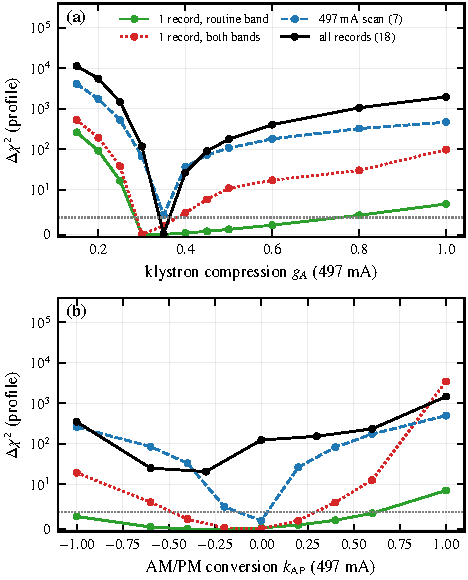
\includegraphics[width=\linewidth]{figures/identifiability}
\caption{Profile likelihood of the klystron's (a) amplitude compression $\gA$ and (b) AM/PM conversion $\kAP$ at the \SI{497}{mA} operating point, with both free at every operating point, for nested data sets: the loop band of one record (\SIrange{\fSplit}{\fHi}{kHz}), the same record over the full band, the gain and phase scan at \SI{497}{mA}, and all records. Every other parameter is re-optimized at each point; the dotted line marks the 95\% level ($\Delta\chi^2=3.84$). The vertical axis is linear below 10.}\label{fig:ident}
\end{figure}

\subsection{What the trip records add}\label{sec:trips}

The trip records measure the klystron without any loop model (App.~\ref{app:trips}). In the normal operation before each trip, the relative fluctuations of the klystron output amplitude follow those of the drive amplitude with a ratio of $\tripGA\pm\tripGAErr$ between 50 and \SI{200}{kHz} over the \tripUsed{} records (Fig.~\ref{fig:trips}a): $\tripGAFull\pm\tripGAFullErr$ at full output and $\tripGARed\pm\tripGARedErr$ at the no-beam output. The coherence is \tripCohLo--\tripCohHi, and the $H_2$ estimate, biased the other way by noise, gives \tripGAHtwo, so the ratio is the klystron's small-signal compression $\gA$. Below \SI{10}{kHz} it is \tripGALow, and above \SI{200}{kHz} it falls to $\tripGAHigh\pm\tripGAHighErr$, where the two measurement chains need not be flat. The probe's response to drive amplitude, relative to its response to drive phase, gives the AM/PM conversion: for a memoryless klystron and any plant that treats both quadratures alike the ratio is $\kAP-j\gA$, and the records give $\kAP=\tripKAP\pm\tripKAPErr$ (Fig.~\ref{fig:trips}b). The loop's own correlation pulls this ratio towards a linear klystron---the same regression returns $\gA=\tripGARatio$ instead of \tripGA---so $|\kAP|$ is if anything underestimated, by about a fifth. The values that the closed-loop records give with $\kAP$ free at every operating point, from \kapFreeLo{} to \kapFreeHi, lie far outside this range.

We therefore fix the AM/PM conversion at the trip-record value. This raises $\chi^2$ by \chiCostKap, \SI{\chiCostKapPct}{\percent} of its value, moves the compression at full current by at most \gaShiftHigh, and leaves the nuisance parameters regular: the noise angle, which depends only on the klystron's insertion phase, varies by \ang{\alphaSpread} between operating points instead of \ang{\alphaSpreadFree}.

\begin{figure*}[tb]
\centering
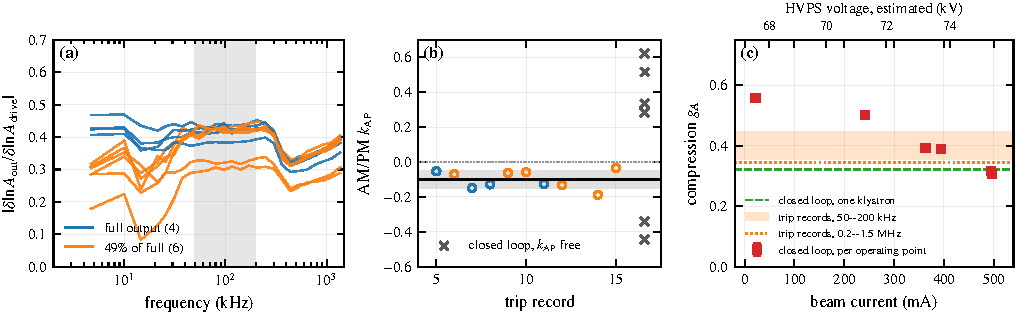
\includegraphics[width=\textwidth]{figures/trip_klystron}
\caption{The klystron in the trip records (present tube, 2021). (a) Ratio of the relative fluctuations of output and drive amplitude against frequency, for the records at full output (blue) and at the no-beam output (orange); shaded: \SIrange{50}{200}{kHz}. (b) AM/PM conversion from the probe's response to drive amplitude and phase, per record (band: mean $\pm$ standard deviation); crosses: the values of the closed-loop fit with $\kAP$ free at every operating point. (c) Compression identified from the closed-loop records at each operating point (squares) and as one value for all currents (dashed), against the trip records at \SIrange{50}{200}{kHz} (band) and above \SI{200}{kHz} (dotted); top axis: HVPS voltage estimated from the power balance at the fixed drive.}\label{fig:trips}
\end{figure*}

% ======================================================================================================
\section{Competing explanations}\label{sec:explain}
% ======================================================================================================

\subsection{The anomaly}

Fitted record by record with a complex-linear loop, the loop band of every record is described to within a few percent ($\chi^2/\nu=\chiLoopLinEff$), but the parameters drift with the operating point (Fig.~\ref{fig:effective}). At the operating gain setting, the effective loop gain falls from \effGLow{} at \SI{22}{mA} to \effGHigh{} at \SI{500}{mA}; the effective delay rises from \SI{\effTauLow}{ns} to \SIrange{\effTauHighLo}{\effTauHighHi}{ns}; the effective $\QL$ falls from about \effQLow{} to \effQHighLo--\effQHighHi. None of these is plausible for the hardware: the gain is held by gain tracking, the delay is cable and klystron transit time and was measured as \SI{\tauMeas}{ns}, and $\QL$ is fixed by the couplers and agrees at low current with the value from the reflected power. At \SI{497}{mA} the effective gain also scales more steeply than the gain setting, and at \SI{22}{mA} it changes with the phase setting---from \effGPhaseA{} to \effGPhaseB{} as the phase setting is lowered by \ang{\phaseScanLow}---which no rotation can do. The same records show the coupled beam mode as a resonance near $\pm f_s$ whose frequency falls from \modeFreeFHi{} to about \SI{\modeFreeFLo}{kHz} with current, and whose damping rate rises from about \SI{\dampHighGainFree}{} to \SI{\dampLowGainFree}{s^{-1}} as the gain is lowered by \SI{1.5}{dB} at \SI{497}{mA} (Fig.~\ref{fig:data}).

\begin{figure*}[tb]
\centering
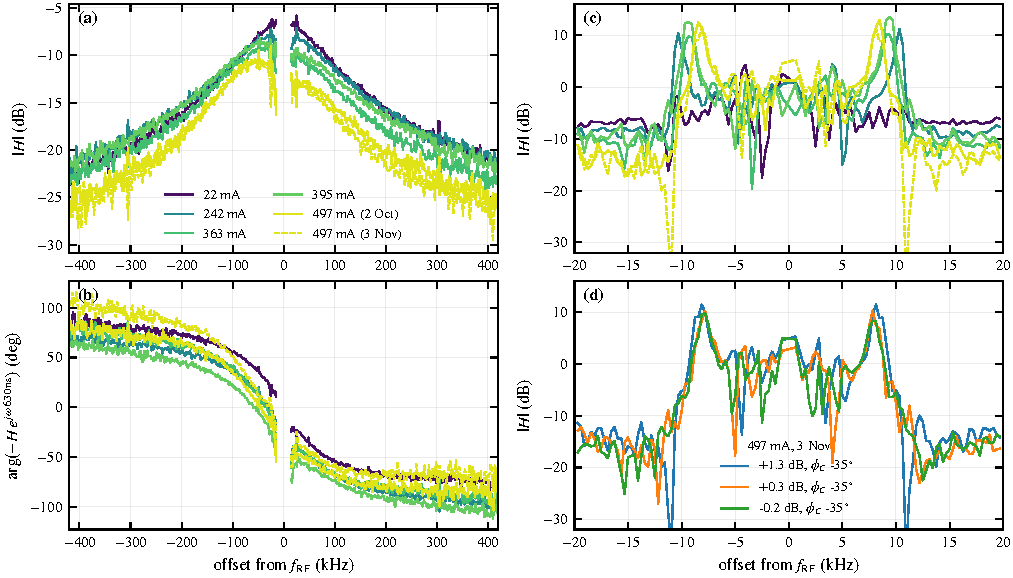
\includegraphics[width=\textwidth]{figures/data_overview}
\caption{Measured closed-loop responses, independent LPM estimates every \SI{\lpmWidth}{Hz} combined into data points as in the fits, through the carrier. (a) Magnitude and (b) phase over the full band (logarithmic offset axis, linear within \SI{0.5}{kHz}), the phase with \SI{630}{ns} of delay removed; colour: beam current; (I), (II): sessions. (c) The near band for the same records: the coupled mode appears as a resonance near $\pm f_s$ that moves down with current. (d) The near band at \SI{497}{mA} (session II) for three loop-gain settings, relative to the operating setting. Dotted: noise level, the standard deviation of the estimates, at 22 and \SI{497}{mA} (II) in (a) and (c) and for one record in (d); where it approaches $|H|$, near the carrier, the estimates scatter accordingly.}\label{fig:data}
\end{figure*}

\begin{figure*}[tb]
\centering
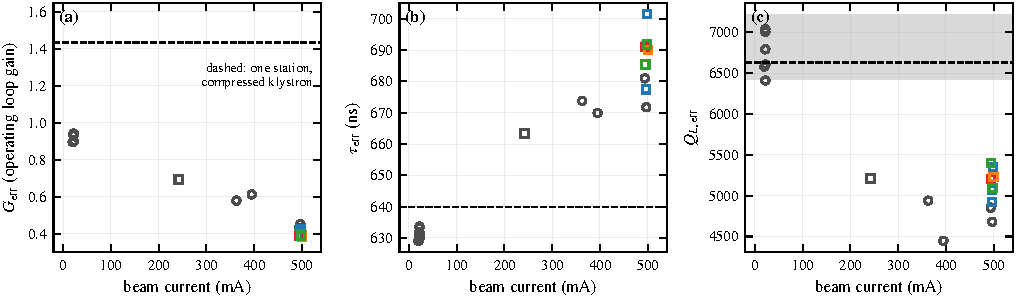
\includegraphics[width=\textwidth]{figures/effective_parameters}
\caption{Effective parameters of record-by-record complex-linear fits: (a) loop gain at the operating gain setting, (b) loop delay, (c) loaded $Q$. Circles: session I; squares: session II, coloured at \SI{497}{mA} by the loop-gain setting as in Fig.~\ref{fig:mode}(b). Dashed: the station constants of the selected model (Sec.~\ref{sec:selected}); grey band in (c): $\QL$ of the four cavities from their reflected power.}\label{fig:effective}
\end{figure*}

\subsection{Explanations and their test}

Table~\ref{tab:models} compares the candidate explanations, each fitted to all eighteen records over the full band (\nPoints{} real data points).
\begin{itemize}
\item \emph{One station, linear klystron.} Shared hardware, detuning from the data, beam dynamics included. It fails by more than an order of magnitude in both bands: the change of the response with current is not a beam-dynamics effect at fixed hardware.
\item \emph{Unequal cavity detunings.} A spread of the four detunings broadens the vector-sum response and could mimic a lower $\QL$. Fitted freely it reaches spreads of tens of kilohertz, which the measured reflected power of every cavity (1--3\%) excludes, and it still fails.
\item \emph{Effective parameters per record.} Per-record $G$, $\tau$ and $\QL$ describe the loop band as well as any model here ($\chi^2/\nu=\chiWideEff$) but not the near band (\chiBeamEff): at the coupled mode, between 5 and \SI{15}{kHz}, they leave \chiEffMode{} times the noise variance, against \chiSelMode{} for the selected model, because the damping of the coupled mode they imply is too small. They also lack a physical reading and do not transfer between conditions (Sec.~\ref{sec:valid}).
\item \emph{Compressed klystron.} Shared hardware, the klystron's compression and the noise angle per operating point, its AM/PM conversion from the trip records. With the momentum compaction identified (Sec.~\ref{sec:fs}) it describes the near band at the noise level ($\chi^2/\nu=\chiBeamSel$) and the loop band to within a few percent of $|H|$ (\chiWideSel) with \nparSel{} parameters; with the design value it fails in the near band and pulls the station constants away from their measured values. Variants test the klystron itself. Its compression and AM/PM taken from the trip records, with no klystron parameter fitted, already describe the records far better than any linear model ($\chi^2/\nu=\chiTrip$). One compression for all currents is worse ($\Delta\mathrm{AIC}=\daicOne$), and freeing the AM/PM conversion at every operating point lowers $\chi^2$ only by the amount discussed in Sec.~\ref{sec:trips}, with values that the trip records exclude. Without the beam's dipole motion the fit fails by far ($+\daicNobeam$).
\end{itemize}

\begin{table*}[tb]
\caption{Candidate explanations fitted to all records over the full band. The compressed-klystron models use the AM/PM conversion of the trip records unless stated. $n_p$: free parameters; $\chi^2/\nu$ overall and in the loop band (\SIrange{\fSplit}{\fHi}{kHz}) and the near band ($|f|<\SI{\fSplit}{kHz}$); $\Delta$AIC and $\Delta$BIC relative to the selected model~\cite{Akaike1974,Schwarz1978}.}\label{tab:models}
\begin{ruledtabular}
\begin{tabular}{lrrrrrr}
Model & $n_p$ & $\chi^2/\nu$ & loop band & near band & $\Delta$AIC & $\Delta$BIC \\
\hline
One station, linear klystron & \nparShared & \chiShared & \chiWideShared & \chiBeamShared & \daicShared & \dbicShared \\
\quad + unequal cavity detunings & \nparSpread & \chiSpread & \chiWideSpread & \chiBeamSpread & \daicSpread & \dbicSpread \\
Effective $G$, $\tau$, $\QL$ per record & \nparEff & \chiEff & \chiWideEff & \chiBeamEff & \daicEff & \dbicEff \\
Klystron of the trip records, none fitted & \nparTrip & \chiTrip & \chiWideTrip & \chiBeamTrip & \daicTrip & \dbicTrip \\
Compressed klystron, one for all currents & \nparOne & \chiOne & \chiWideOne & \chiBeamOne & \daicOne & \dbicOne \\
Per operating point, design $\alpha_c$ & \nparSelNom & \chiSelNom & \chiWideSelNom & \chiBeamSelNom & \daicSelNom & \dbicSelNom \\
Per operating point, no beam motion & \nparNobeam & \chiNobeam & \chiWideNobeam & \chiBeamNobeam & \daicNobeam & \dbicNobeam \\
Per operating point, AM/PM free & \nparFree & \chiFree & \chiWideFree & \chiBeamFree & \daicFree & \dbicFree \\
\textbf{Selected: compression per operating point} & \nparSel & \chiSel & \chiWideSel & \chiBeamSel & 0 & 0 \\
\end{tabular}
\end{ruledtabular}
\end{table*}

\begin{figure*}[tb]
\centering
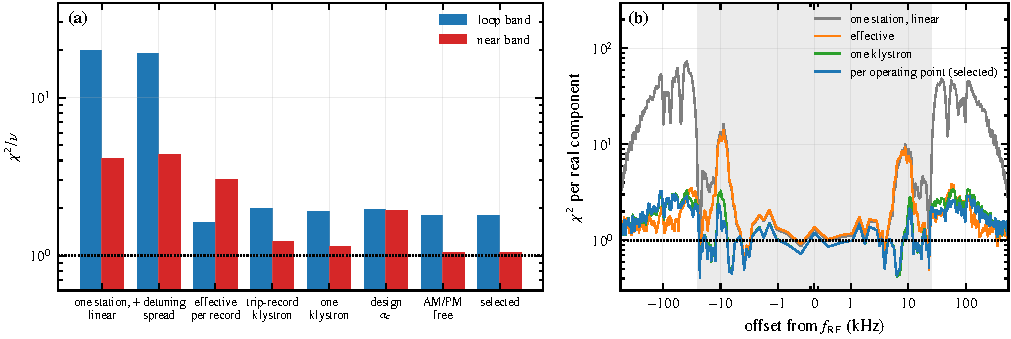
\includegraphics[width=\textwidth]{figures/model_comparison}
\caption{(a) $\chi^2/\nu$ of the candidate explanations of Table~\ref{tab:models} in the loop band and the near band (all records); the last three have the compression per operating point. (b) Squared normalized residuals per real component over the full band (shaded: near band), averaged over all records and over five adjacent data points; 1 is the noise level. The dips near $\pm\SI{22}{kHz}$ lie at interference lines, which raise the averaged noise level there.}\label{fig:models}
\end{figure*}

Figure~\ref{fig:models}(b) shows where the models fail. The linear station misses everywhere. In the near band the selected model is close to the noise level for every record ($\chi^2/\nu$ of \chiRecNearLo--\chiRecNearHi), the coupled mode included. In the loop band every model with a compressed klystron, and the effective model with three free parameters per record, leaves the same residual structure, a few percent of $|H|$ with opposite signs on the two sides of the carrier; it is largest between 25 and \SI{150}{kHz} ($\chi^2/\nu=\chiSelLoopLow$ for the selected model) and smaller above (\chiSelLoopHigh). It is worst in the two extreme settings of the low-current phase scan ($\chi^2/\nu$ of \chiRecLowLo{} and \chiRecLowHi{} over the full band, against at most \chiRecOthersHi{} and a median of \chiRecOthersMedian{} for the other records). Two physical causes were tested and rejected. A finite bandwidth of the klystron's amplitude path alone, between \fAlo{} and \SI{\fAhi}{MHz} with the phase path unchanged, worsens the fit by at least $\Delta\chi^2=\dchiFAmin$, so the fall of the trip-record compression above \SI{200}{kHz} (Sec.~\ref{sec:trips}) more likely belongs to the measurement chains than to the tube; and unequal loaded $Q$ of the four cavities, taken from their reflection (spread \qSpread\%), changes $\chi^2$ by \dchiQrel. The structure is common to all the explanations compared here and does not decide between them; it sets the accuracy of the model in the loop band.

\subsection{The selected model}\label{sec:selected}

The station constants are $G_0=\Gzero\pm\GzeroErr$, $\tau=\tauFit\pm\tauFitErr$~ns and $\QL=\QLFit\pm\QLFitErr$ (statistical errors). The delay is \SI{\tauDiff}{ns} longer than the \SI{\tauMeas}{ns} measured on the station~\cite{Sebek2026}, a difference that the excitation and recording paths outside the loop can account for: their linear phase is absorbed in $\tau$ (Sec.~\ref{sec:model}). $\QL$ lies within the range of the four cavities' loaded $Q$ from their reflection without beam (\QLreflLo--\QLreflHi, \QLrefl{} for their vector sum; Sec.~\ref{sec:system}). The measurement chain contributes an odd magnitude slope of \chainOdd~dB and an even phase of \ang{\chainEvenPh} at $\pm\SI{400}{kHz}$, common to all records. Table~\ref{tab:groups} lists the operating-point parameters. The detunings follow the beam-loading compensation, $\Delta f\approx-\SI{36}{kHz}\times\Ib/\SI{500}{mA}$, to within about \SI{3}{kHz}, as the tuners' load-angle offset allows. The loop phase at \SI{22}{mA} follows the phase setting with a slope of \thetaSlopeLow{} degrees per degree.

The klystron's compression grows with the beam current, from $\gA=\gaSelLow$ at \SI{22}{mA} through \gaSelMid{} at 242, 363 and \SI{395}{mA} to \gaSelHighLo--\gaSelHighHi{} at \SI{494}{}--\SI{497}{mA}, and the two high-current operating points, measured a month apart, agree within their errors. This is the trend that the station's operation implies: the drive is the same at every current, but with beam the tube runs at a higher voltage and much closer to saturation (efficiency \SI{\klyEffHigh}{\percent} against \SI{\klyEffLow}{\percent} without beam, Sec.~\ref{sec:system}). The HVPS voltage was not recorded with the closed-loop records. Estimated from the power balance at the fixed drive---cavity losses, beam power and the reflection at the cavities' coupling $\beta\approx\betaMean$, scaled by \pfwdScale{} to the snapshots and interpolated between their voltages---it rises from about \SI{\vkLow}{kV} at \SI{22}{mA} through \vkMid{}~kV to \SI{\vkHigh}{kV} at \SI{494}{}--\SI{497}{mA} (Table~\ref{tab:groups}), and the compression falls monotonically with it. The phase path of the loop therefore has the gain $G_0=\Gzero$ at the operating setting, while a perturbation of the drive amplitude meets a loop gain of only $\gA G_0\approx\ampLoopHigh$ at \SI{500}{mA}. The effective loop gain of about \effGLow{} that a complex-linear fit returns at low current (Fig.~\ref{fig:effective}a) is neither of the two but their projection on the direction of the injected noise [Eq.~\eqref{eq:recorded}].

\begin{table*}[tb]
\caption{Records and operating-point parameters of the selected model. Sessions I and II were a month apart; $n$: number of records; $\Delta G$, $\Delta\phi$: loop-gain and loop-phase settings relative to the operating settings; $V_k$: HVPS voltage, not recorded, estimated from the power balance at the fixed drive (Sec.~\ref{sec:selected}); $\gA$: klystron compression (statistical errors); $\alpha$: noise angle in the cavity frame; $\Delta f$: detuning of each group of records taken minutes apart. The AM/PM conversion is fixed at $\kAP=\kapTrip$ (trip records, Sec.~\ref{sec:trips}).}\label{tab:groups}
\begin{ruledtabular}
\begin{tabular}{lcccccccc}
Session & $\Ib$ (mA) & $n$ & $\Delta G$ (dB) & $\Delta\phi$ ($^\circ$) & $V_k$ (kV) & $\gA$ & $\alpha$ ($^\circ$) & $\Delta f$ (kHz) \\
\hline
I & 22 & 6 & $-0.4$ & $-3$ to $+6$ & 67 & $0.56\pm0.01$ & $-12$ & $-1.9$, $-1.8$, $+1.0$ \\
I & 363 & 1 & $-0.4$ & $-3$ & 73 & $0.40\pm0.01$ & $-16$ & $-24.2$ \\
I & 395 & 1 & $-0.4$ & $+0$ & 74 & $0.39\pm0.01$ & $-23$ & $-27.9$ \\
I & 496 & 2 & $-0.4$ & $-3$ to $+0$ & 75 & $0.32\pm0.01$ & $-11$ & $-33.1$ \\
II & 242 & 1 & $+0.0$ & $+0$ & 71 & $0.49\pm0.01$ & $-14$ & $-18.2$ \\
II & 497 & 7 & $-1.5$ to $+0.0$ & $-15$ to $-10$ & 75 & $0.31\pm0.01$ & $-4$ & $-33.2$

\end{tabular}
\end{ruledtabular}
\end{table*}

\begin{figure*}[tb]
\centering
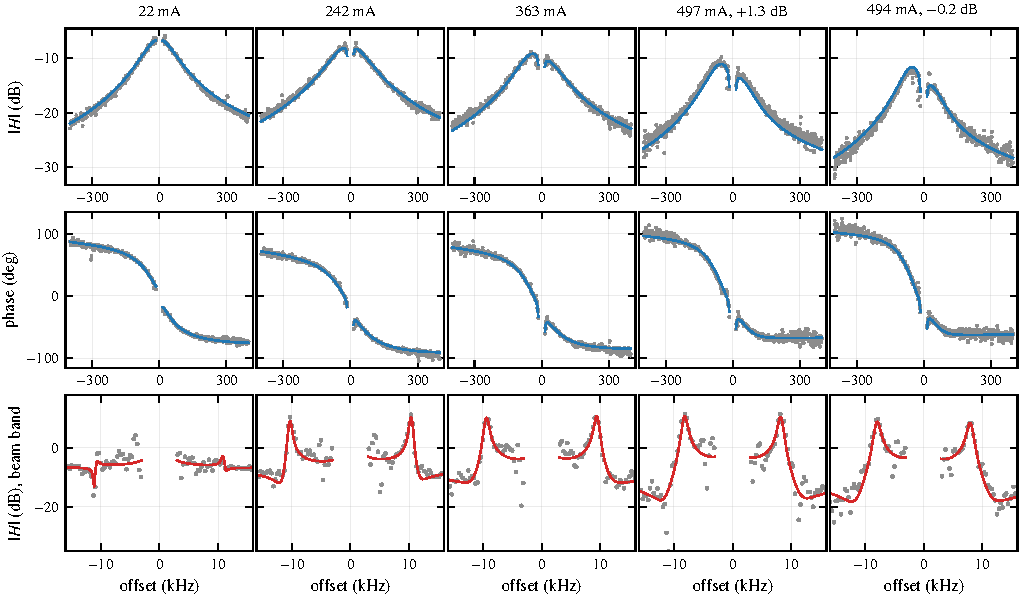
\includegraphics[width=\textwidth]{figures/fits}
\caption{Recorded responses (grey) and the selected model (lines) for five operating points, labelled by beam current and, at \SI{497}{mA} (session II), loop-gain setting: magnitude and phase over the full band (top, middle; phase with \SI{630}{ns} removed) and magnitude in the near band (bottom; shaded: the model $\pm$ the standard deviation of the estimates, the scatter expected of the data). The model is averaged over the \SI{\lpmWidth}{Hz} of each estimate. One set of station constants describes all records.}\label{fig:fits}
\end{figure*}

% ======================================================================================================
\section{Validation}\label{sec:valid}
% ======================================================================================================

\subsection{Out-of-band prediction of the coupled mode}\label{sec:fs}

The first test asks whether the loop identified in the loop band alone predicts the coupled mode, which lives in a band that was not used. For each of the \nModeRecs{} records with more than \SI{200}{mA}, the coupled mode is measured without a model by fitting a pole pair and a smooth background to both sides of the near band between 3 and \SI{16}{kHz} (App.~\ref{app:estimator}); frequencies are determined to about \SI{\modeFreeDf}{Hz} and damping rates to about \SI{\modeFreeDs}{s^{-1}}. The models are then evaluated with no adjustment.

Both loop-band models fail, in opposite ways (Fig.~\ref{fig:mode}a). The effective linear model places the mode at about the right frequency (mean error \oobEffDf~Hz) but with too little damping (mean error \oobEffDs~s$^{-1}$, rms \oobEffDsRms~s$^{-1}$): its effective parameters describe the projection that the routine measures, not the impedance that the beam sees. The compressed-klystron model gets the damping roughly right (mean error \oobWlDs~s$^{-1}$)---the klystron's compression supplies the damping that a linear model lacks---but places the mode \oobWlDfAbs~Hz too low. The prediction thus isolates one discrepancy, the coherent frequency, in a model whose loop is otherwise right.

The coherent frequency at fixed loop depends on the beam through $\omega_s^2$ and $\kappa_1I_{b1}$, both proportional to $\alpha_c$. The mode at \SI{242}{mA}, at \modeFreeFHi~kHz, already lies above the nominal incoherent frequency $f_s=\fsNom$~kHz, whereas in every model considered here the reactive loading of cavities tuned below $\fRF$ pulls the coherent mode below $f_s$. Identifying $\alpha_c$ jointly with the loop, from the full band, gives $\alpha_c=\alphacFit\times10^{-3}$, with a statistical error of \alphacFitErr$\times10^{-3}$ and a range of \alphacLo--\alphacHi$\times10^{-3}$ over the compressed-klystron models of Table~\ref{tab:models} that leave it free, i.e., an incoherent synchrotron frequency of \fsFit~kHz at \SI{2.85}{MV} (\fsLo--\fsHi~kHz), \fsRatio\% above the nominal value. With the design value the fit worsens in both bands ($\chi^2/\nu=\chiWideSelNom$ and \chiBeamSelNom{} against \chiWideSel{} and \chiBeamSel), and the station constants move away from their measured values ($\QL=\QLSelNom$, $\tau=\SI{\tauSelNom}{ns}$). Two alternatives were tested. Freeing the beam-coupling strength separately from $\omega_s$ returns a coupling factor $\kscale\pm\kscaleErr$ with $\alpha_c=\alphacKs\times10^{-3}$: both scale as $\alpha_c$ does, which a calibration error of the gap voltage (acting on $\omega_s$ alone) would not produce. And the effective linear model does not improve with $\alpha_c$ free: its deficit is the damping. With $\alpha_c$ identified the coupled mode agrees with the model-free poles to \jointDfRms~Hz in frequency and \jointDsRms~s$^{-1}$ in damping (rms over \nModeRecs{} records), across currents from 242 to \SI{500}{mA} and loop-gain settings down to \SI{\gainDropMax}{dB} below the operating setting (Fig.~\ref{fig:mode}); with one compression for all currents the damping comes out \jointOneDsAbs~s$^{-1}$ too high on average. The identified value lies \alphacAboveLo--\alphacAboveHi\% above the published lattice values, $1.18\times10^{-3}$ for the operating lattice~\cite{Huang2007} and $1.13\times10^{-3}$ in the design report~\cite{Hettel2002}; it is either a property of the present lattice or a proxy for an unmodelled element that acts on the coupled mode like a stronger synchrotron focusing. A direct measurement of the incoherent synchrotron frequency at a few milliamperes, where the coherent shift vanishes, decides between the two: the model predicts \fsFit~kHz.

\begin{figure*}[tb]
\centering
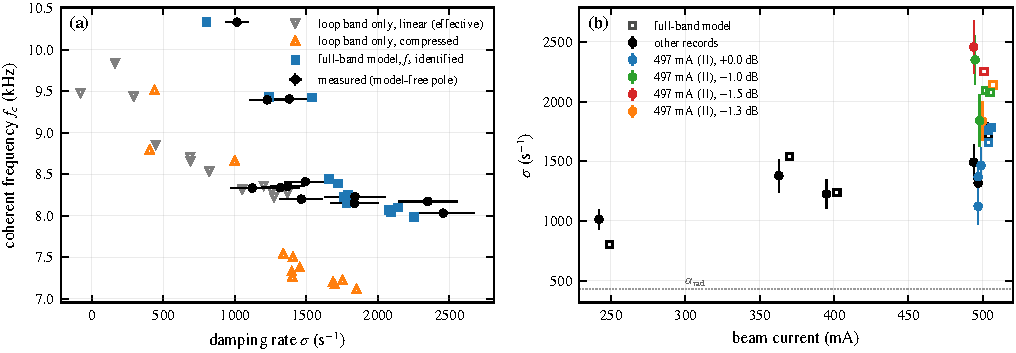
\includegraphics[width=\textwidth]{figures/coupled_mode}
\caption{The coupled beam--cavity--klystron--loop mode. (a) Frequency and damping rate measured without a model (black, $1\sigma$ errors), predicted from the loop band alone by the effective linear model (grey) and by the compressed-klystron model with nominal ring parameters (orange), and given by the full-band model with the synchrotron frequency identified (blue). (b) Damping rate against beam current, measured (filled) and from the full-band model (open squares); at \SI{497}{mA} (session II) the colours mark the loop-gain setting relative to the operating setting. Dotted: radiation damping.}\label{fig:mode}
\end{figure*}

\subsection{Prediction across operating conditions}

The second test asks whether the identified model predicts records taken under conditions it was not trained on. Each model is refitted without the held-out records; for these only nuisance parameters are refitted: the loop phase, plus the detuning (and the noise angle, for the klystron models) when the beam current is new. The effective model needs its per-record parameters at the new condition: they are taken from the same operating point and scaled with the gain setting (gain transfer), averaged over the neighbouring phase settings (phase transfer), or interpolated in beam current (current transfer); the selected model interpolates $\gA$ in beam current, and the single klystron needs nothing. Figure~\ref{fig:crossval} shows the held-out $\chi^2/\nu$.

For a new beam current the selected model predicts the record almost as well as it fits it in sample: \cvIaSel, \cvIbSel{} and \cvIcSel{} at 242, 363 and \SI{395}{mA}, against \cvIaIn, \cvIbIn{} and \cvIcIn{} in sample; the single klystron gives \cvIaOne, \cvIbOne{} and \cvIcOne, and interpolated effective parameters give \cvIaEff, \cvIbEff{} and \cvIcEff. For new gain settings at \SI{497}{mA} the selected model gives \cvGainSel{} on average (in sample \cvGainIn) and the scaled effective model \cvGainEff, the difference lying in the near band (\cvGainNearSel{} against \cvGainNearEff{} per record). For new phase settings at \SI{22}{mA} both give about 3 (\cvPhaseSel{} and \cvPhaseEff), close to the selected model's in-sample value of these two records (\cvPhaseIn). Freeing the AM/PM conversion at every operating point changes no prediction materially (\cvIaFree, \cvIbFree, \cvIcFree; \cvGainFree; \cvPhaseFree). The one-station linear model fails every test.

\begin{figure}[tb]
\centering
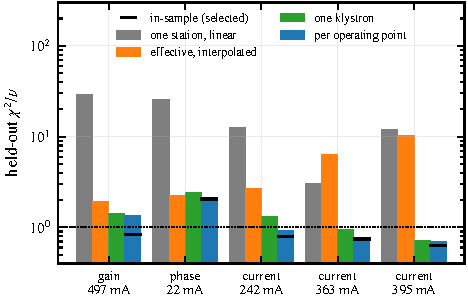
\includegraphics[width=\linewidth]{figures/crossval}
\caption{Held-out $\chi^2/\nu$ (full band) of records predicted from models trained without them: gain transfer at \SI{497}{mA} (four records), phase transfer at \SI{22}{mA} (two), and three beam currents. Bars: one-station linear model, effective model with transferred parameters, one compressed klystron for all currents, compression per operating point (selected). Black ticks: in-sample values of the selected model.}\label{fig:crossval}
\end{figure}

\subsection{Comparison with the trip records}\label{sec:tripcomp}

At full current the identified compression, \gaSelHighLo--\gaSelHighHi{} at \SI{494}{}--\SI{497}{mA} (\gaFreeHigh{} with the AM/PM conversion free), lies below the trip-record value at full output, $\tripGAFull\pm\tripGAFullErr$ at \SIrange{50}{200}{kHz}, and close to the trip-record value above \SI{200}{kHz}, $\tripGAHigh\pm\tripGAHighErr$ (Fig.~\ref{fig:trips}c). Both describe a strongly compressed klystron: a change of the drive amplitude reaches the output with a third to two fifths of its relative size. At low output the two disagree. The trip records give $\tripGARed\pm\tripGARedErr$ at the no-beam output, where the closed-loop records give \gaSelLow{} at \SI{22}{mA}; in the trip records the compression hardly depends on the output, in the closed-loop records it does. A single compression for all currents, \gaOneKly, costs $\Delta\chi^2=\dchiOne$: \dchiOneLow{} from the \SI{22}{mA} records, \dchiOneMid{} from the single records at 242--\SI{395}{mA}, and \dchiOneHigh{} from the eleven records at 494--\SI{497}{mA}. The current dependence thus rests on the low-current phase scan, which no model reproduces at the noise level in its extreme settings, and on the records at intermediate current, among them the near band at 242 and \SI{363}{mA}, where a single compression overestimates the damping. It is the trend expected from the klystron's efficiency at the two voltages (Sec.~\ref{sec:selected}). The trip records are five years older, and their beam currents, cathode voltages and loop settings were not recorded; a transfer-curve measurement at the present drive and at the cathode voltages of low and high current would settle the point. Taken as they are, with no klystron parameter fitted, the trip-record values describe all eighteen records better than any linear model ($\chi^2/\nu=\chiTrip$, Table~\ref{tab:models}).

\subsection{Physical consistency}

The station constants agree with independent knowledge: $\tau$ with the delay measured on the station, to within the delay outside the loop, $\QL$ with the reflected power, the detunings with the beam-loading compensation, the gain constant across operating points with the gain tracking, the loop-phase slope at low current with the earlier calibration, and the growth of the compression with the klystron's efficiency. None of these was imposed.

% ======================================================================================================
\section{Discussion}\label{sec:disc}
% ======================================================================================================

\paragraph{What changes with the beam.} The dominant change of the loop dynamics between \SI{20}{} and \SI{500}{mA} is the compression of the klystron, which runs closer to saturation as the HVPS raises its voltage to supply the beam's power at a fixed drive; the detuning and the beam's dipole motion are the other two current-dependent elements, and both follow from physics once the loop is known. A complex-linear model can follow the change only with effective parameters that mean nothing physical, and such a model does not predict the coupled mode or new operating points. The compression divides the loop into two: a phase loop of gain $G_0\approx\Gzero$ and an amplitude loop of about one third of that at \SI{500}{mA} ($\gA G_0\approx\ampLoopHigh$). The weaker amplitude loop leaves more of the cavity's natural impedance to the beam, and that supplies the Robinson damping that a linear model cannot: identified on the loop band alone, the linear model with effective parameters underestimates the damping of the coupled mode by about \SI{\oobEffDsAbs}{s^{-1}} on average (Sec.~\ref{sec:fs}). Lowering the gain by \SI{1.5}{dB} at \SI{497}{mA} raises the measured damping rate from about \SI{\dampHighGainFree}{} to \SI{\dampLowGainFree}{s^{-1}}; the model reproduces the direction and \dampChangePct\% of the size of this change (\SI{\dampHighGainModel}{} to \SI{\dampLowGainModel}{s^{-1}}), but at the highest gain it overestimates the damping by about \SI{\dampHighGainOver}{s^{-1}}, \dampOverRatio{} times the measurement error.

\paragraph{The synchrotron frequency.} The near band identifies a combination of beam parameters that the loop band cannot, and the result disagrees with the design value by \fsRatio\% in $f_s$. Because the incoherent synchrotron frequency is easy to measure at low current, this is a falsifiable prediction; if it is confirmed, the momentum compaction of the present lattice should be revised in every longitudinal model of the ring; if not, the coupled-mode band contains dynamics that the model lacks, most likely in the integral path or the klystron at a few kilohertz.

\paragraph{Limits.} The model assumes rigid bunches and a uniform fill, equal vector-sum weights and a memoryless klystron, and it treats the measurement chain as a smooth common factor. The loop phase of each record is a free parameter because the tracking correction was not recorded. The AM/PM conversion is taken from trip records five years older than the closed-loop data, because the closed-loop records determine it only together with the high-current loop phase; its value is small, and the compression at full current hardly depends on it. In the loop band the model leaves a residual of a few percent of $|H|$, common to all the explanations tested and largest in the low-current phase scan; neither a finite klystron bandwidth nor unequal cavity $Q$ explains it. Operating-point parameters for currents with a single record rest on that record, and the HVPS voltages of the operating points between \SI{0}{} and \SI{500}{mA} are estimated, not measured.

\paragraph{Measurements that would add most.} A two-dimensional excitation---independent noise sequences on I and Q, or a multisine whose lines sit on one side of the carrier---would measure $H_1$ and $H_2$ separately and determine the AM/PM conversion from the closed-loop records themselves. Longer records, or more excitation within a few kilohertz of the carrier, would raise the signal-to-noise ratio of the near band above the \snrNearLo--\SI{\snrNearHi}{dB} per estimate of these records (Sec.~\ref{sec:estimation}) and sharpen the coupled mode accordingly. The klystron's transfer curves (AM/AM and AM/PM) at the present drive and at the cathode voltages of low and high current would test the identified growth of the compression with current, which the older trip records do not show. Recording the HVPS voltage and the klystron's drive and output power with every closed-loop record would tie each record to its point on those curves, and recording the total loop phase would remove one nuisance parameter per record. The incoherent synchrotron frequency at low current settles the question of $\alpha_c$. With these, the same routine records would give a complete, predictive model of the station---and, for the replacement LLRF system, whose loop delay is longer, a quantitative basis for setting its gain and phase.

% ======================================================================================================
\section{Conclusions}\label{sec:concl}
% ======================================================================================================

Operational closed-loop measurements, taken with an existing diagnostic routine and a one-dimensional excitation, identify a compact physics-informed model of the coupled beam--cavity--klystron--feedback system of the SPEAR3 RF station. One set of station constants---loop gain, delay, loaded $Q$---describes eighteen records from 20 to \SI{500}{mA}, at several loop gains and phases, in two sessions a month apart, once the klystron is allowed to compress its amplitude response as it approaches saturation: at the noise level in the band of the coupled mode and to within a few percent of the response across the loop band. The constants agree with independent station data. Single records do not determine the klystron's asymmetry; records at several loop settings and the near band determine its compression, and trip records of the same tube supply its small AM/PM conversion, which the closed-loop records leave correlated with the loop phase. The compression grows with the beam current as the tube, held at a fixed drive, works closer to saturation; at full current it agrees with the trip records to within their spread across frequency bands, while the trip records show less dependence on the output power. Explanations by effective linear parameters, by unequal cavity detunings, or by beam dynamics at fixed hardware are rejected by the data. The identified model predicts records at beam currents it was not trained on almost at in-sample quality, where interpolated effective parameters fail. Its out-of-band prediction of the coupled beam mode isolated the one beam parameter that the loop band cannot determine; identified from the near band, it implies an incoherent synchrotron frequency \fsRatio\% above the design value, whatever the klystron model, a prediction that a simple low-current measurement can test. The physics supplied the structure; the data determined the klystron's compression, the station constants and the synchrotron focusing, and tested every explanation against measurements it was not built from.


\begin{acknowledgments}
We thank the SSRL operations and RF groups for the closed-loop records, the trip records and the station snapshots on which this study rests. All measurements analyzed here were taken by existing operational routines; no setting of the station was changed for this work.
\end{acknowledgments}

\section*{Data and code availability}
The closed-loop records, trip records and station snapshots, and the analysis code that produces every figure and every number in the text, are available from the authors on reasonable request.

\appendix
% ======================================================================================================
\section{Beam-loaded plant and recorded response}\label{app:derivation}
% ======================================================================================================

With the cavity voltages $\vect v_k=\mat Z_k(\vect i_g-I_{b1}\hat{\vect b}\,\Delta\phi)$ and Eq.~\eqref{eq:beam},
\begin{equation}
\Bigl(s^2+2\arad s+\omega_s^2\Bigr)\Delta\phi=\kappa_1\hat{\vect p}^\mathsf{T}\mat Z_\Sigma\vect i_g-\kappa_1I_{b1}\bigl(\hat{\vect p}^\mathsf{T}\mat Z_\Sigma\hat{\vect b}\bigr)\Delta\phi ,
\end{equation}
so $\Delta\phi=\kappa_1\hat{\vect p}^\mathsf{T}\mat Z_\Sigma\vect i_g/D(s)$ and $\vect v_m=\mat Z_m\vect i_g-I_{b1}\mat Z_m\hat{\vect b}\,\Delta\phi$ gives Eq.~\eqref{eq:plant}. The term $\kappa_1I_{b1}\hat{\vect p}^\mathsf{T}\mat Z_\Sigma\hat{\vect b}$ equals $-j\kappa[Z_\Sigma(s)-\bar Z_\Sigma(s)]$ with $\kappa=\kappa_1I_{b1}/2$, so that $D(s)$ is the open-loop characteristic function of the beam-loaded cavity~\cite{Pedersen1975}; multiplied by the cavity denominator it is Pedersen's quartic.

The loop of Eq.~\eqref{eq:loop} places the klystron between the drive chain and the cavities. Blocks with a real impulse response commute with every $2\times2$ matrix, so only the order of the rotation $\mat R(\theta)$, the plant $\mat P_b$ and the klystron $\mat K$ matters. The noise is injected into the drive in the RFP frame; with $\psi$ the phase from the RFP drive frame to the cavity frame, conjugating every signal by $\mat R(\psi)$ moves the loop to the cavity frame and turns the injection angle $\alpha_\mathrm{RFP}$ into $\alpha=\alpha_\mathrm{RFP}+\psi$. The loop phase $\theta$ includes $\psi$ and the controller rotation; a change of the loop-phase setting changes $\theta$ but not $\alpha$, while a change of the klystron's insertion phase with its cathode voltage changes both.

If the excitation is one-dimensional, with a real amplitude $r(t)$ along a fixed angle $\alpha$, $\vect n(t)=r(t)(\cos\alpha,\sin\alpha)^\mathsf{T}$, the complex input is $n=e^{j\alpha}r$ and $\overline{n(-f)}=e^{-2j\alpha}n(f)$; the widely linear output $x=H_1n+H_2\overline{n(-f)}$ is then $(H_1+H_2e^{-2j\alpha})\,n$, Eq.~\eqref{eq:recorded}. The recorded response is fully coherent with the reference, but it is one projection: $H_1$ and $H_2$ cannot be separated from one record, and parameters that act only through the image response $H_2$---the klystron's asymmetry above all---are confounded with the loop parameters (Sec.~\ref{sec:ident}).

The closed-loop poles are the zeros of $\det[\mat 1+\mat M(s)]D(s)$. With $\mat F=\mat K\,Gc\,\mat R(\theta)/R_L$, Sylvester's identity gives $\det(\mat 1+\mat M)=\det(\mat 1+\mat F\mat P_b)$, and since $\mat P_b$ is $\mat Z_m$ minus a rank-one term, the matrix determinant lemma gives the exact factorization
\begin{equation}
\det[\mat 1+\mat M(s)]\,D(s)=\det(\mat 1+\mat F\mat Z_m)\,D_0(s),
\end{equation}
where $D_0(s)=s^2+2\arad s+\omega_s^2+\kappa_1I_{b1}\hat{\vect p}^\mathsf{T}\mat Z_b\hat{\vect b}$ is the characteristic function of the beam with the closed-loop impedance $\mat Z_b=\mat Z_\Sigma(\mat 1+\mat F\mat Z_m)^{-1}$ that feedback presents to it~\cite{Boussard1985,Wilson1993}, and $\det(\mat 1+\mat F\mat Z_m)$ that of the RF loop without beam. The coupled mode is tracked by Newton continuation from $\Ib=0$, where it is the incoherent oscillator $s=-\arad\pm j(\omega_s^2-\arad^2)^{1/2}$.

% ======================================================================================================
\section{Estimator statistics}\label{app:estimator}
% ======================================================================================================

With the bin offset $r=-n,\dots,n$ ($n=4$) around a centre bin $k$, the LPM fits
\begin{equation}
Y_{k+r}=\hat G\,X_{k+r}+\sum_{q=0}^{2}t_q\,(r/n)^q+E_r
\end{equation}
by least squares~\cite{Pintelon2010}, i.e.\ $\vect Y=\mat K\vect\vartheta+\vect E$ with $\vect\vartheta=(\hat G,t_0,t_1,t_2)^\mathsf{T}$ and $\hat G=\vect e_0^\mathsf{T}(\mat K^\mathsf{H}\mat K)^{-1}\mat K^\mathsf{H}\vect Y$. The neighbourhoods tile the spectrum outward from the carrier; in the one centred on it, the carrier bin, which holds the record's mean, is left out of the fit. Any quadratic transient is annihilated, and with Eq.~\eqref{eq:lpm} the expectation of the estimate is
\begin{align}
\langle\hat G\rangle&=\sum_r c_r\,G_{k+r},\\
\vect c^\mathsf{T}&=\vect e_0^\mathsf{T}(\mat K^\mathsf{H}\mat K)^{-1}\mat K^\mathsf{H}\,\mathrm{diag}(X_{k+r}),
\end{align}
with weights that sum to one; for output noise of variance $\sigma_V^2$ per bin its variance is $\sigma_V^2[(\mat K^\mathsf{H}\mat K)^{-1}]_{00}$. The noise variance is estimated from the residual of the same fit with $G$ quadratic as well (six unknowns, three degrees of freedom), $s_k^2=\sum_r|E_r|^2/3$, averaged over \SI{\lpmSmooth}{kHz}. Holding $G$ constant in the estimate costs no variance and causes no bias, because the model is averaged with the same weights $c_r$; this matters near the coupled mode, where the response changes within one neighbourhood. In the loop band, where several estimates form one data point, the model is evaluated at their weighted mean frequency.

The predicted variance is tested without a model on the scatter of adjacent estimates about a linear trend. Above \SI{100}{kHz}, in groups of eight (\SI{2.8}{kHz}), the weighted residual is \calibMedian{} times its expectation (median over the records; \calibLo--\calibHi). In the near band, in groups of four, the ratio lies between \calibNearLo{} and \calibNearHi: interference lines near $\pm22$ and $\pm\SI{27}{kHz}$ raise the averaged noise level of the estimates around them, which therefore weigh less, and below \SI{5}{kHz} the response itself curves within a group. Within \SI{3}{kHz} of the carrier, where the noise level changes fast and the harmonics of the high-voltage ripple (multiples of \SI{720}{Hz}) stand out, the averaged level is too low on the estimates that contain a harmonic and too high on the others: there the residuals of the selected model are \nearCalLo{} to \nearCalHi{} times their predicted standard deviation (median over the records). Averaging the noise level over fewer bins does not remove this and makes the level itself noisier. The Welch estimate that the routine uses has the right variance per bin, but adjacent bins of overlapping segments are correlated and its resolution is set by the segment length; treating its bins as independent overstates the information they carry, and near the coupled mode the model has to be convolved with the window. The LPM uses the whole record, removes the transient and gives independent estimates.

The model-free estimate of the coupled mode fits, on both sides of the carrier at once (3 to \SI{16}{kHz}), a smooth background (complex quadratic in $f$) plus the residues of one complex pole pair $s=-\sigma\pm j\omega_c$, each averaged with the weights $c_r$ of the estimates.

% ======================================================================================================
\section{Trip records}\label{app:trips}
% ======================================================================================================

At a trip the station's fast acquisition memories freeze at the fault and are written to files. Each of the \tripN{} records of 2021, all of the present tube, holds \num{51200} samples per signal at \SI{10.24}{MS/s}, the \SI{5.0}{ms} before the fault. The signals are the klystron drive and one cavity probe, both as I/Q, and the klystron output, whose amplitude $(I^2+Q^2)^{1/2}$ is linear in the RF amplitude. As for the closed-loop records, the stored I/Q are the complex conjugate of the physical envelope: conjugated, the drive-to-probe response places the cavities below $\fRF$ in every record, its phase-path response being \tripAsymLo--\tripAsymHi{} times larger at \SIrange{-45}{-20}{kHz} than at \SIrange{20}{45}{kHz}. In \tripUsed{} records every signal holds RF; in the others some or all of them are empty. The analysis uses the normal operation up to \SI{0.5}{ms} before the end of each record, earlier if any signal leaves its level first.

The compression is the cross-spectrum of the relative output amplitude with the relative drive amplitude over the drive's auto-spectrum ($H_1$; 2048-point Hann segments with \SI{50}{\percent} overlap), with the ratio of the output's auto-spectrum to the cross-spectrum ($H_2$) as the bound from the other side; the two acquisition channels differ in timing by \SI{\tripDelay}{ns}, which only turns the phase of the ratio. For the AM/PM conversion the relative fluctuation $c$ of the probe is regressed, bin by bin (1024-point segments), on the relative drive amplitude $a_d$ and the drive phase $\varphi_d$: $c=A\,a_d+B\,\varphi_d$. For a memoryless klystron $c=P[(\gA+j\kAP)\,a_d+j\varphi_d]$ for any complex-linear plant $P$, so that $A/B=\kAP-j\gA$ whatever the cavities and their detuning; the beam acts on the probe only near $\pm f_s$, outside the band of \SIrange{60}{250}{kHz} used. Feedback correlates the drive with disturbances of the probe and pulls the ratio towards that of a linear klystron ($A/B\to-j$); the compression the regression returns, \tripGARatio{} against \tripGA{} measured directly, gauges that pull.


\bibliography{refs}

\end{document}
